%%%%%%%%%%%%%%%%%%%STETTINGS%%%%%%%%%%%%%%%%%%%%%%%%%%%%%%
\documentclass[12pt]{report}
\usepackage{hyperref}
\usepackage[style=verbose, autocite=footnote, backend=biber]{biblatex}
\addbibresource{ref.bib} 
\usepackage{graphicx} 
\usepackage[utf8]{inputenc}
\usepackage[T1]{fontenc}
%\usepackage[french]{babel}
\usepackage[greek,french]{babel}
\usepackage[margin=2.5cm, left=3.5cm]{geometry}
\usepackage{setspace}
\usepackage{titlesec}
\usepackage{comment}
\usepackage[export]{adjustbox}
\usepackage{pdfpages}


%%%%%%%%%%%%%%%%%%%%%%%%%%%%%%%%%%%%%%%%%%%%%%%%%%%%%%%%
	\titleformat{\section}{}{}{0em}{\bf\LARGE}
	\titleformat{\subsection}{}{}{0em}{\bf\Large}
	\titleformat{\subsubsection}{}{}{0em}{\bf\normalsize}
 
\titleformat{\chapter}[hang]{\bf\huge}{\thechapter}{2pc}{}


%%%%DOCUMENT%%%%

%%\setcounter{tocdepth}{6}
\begin{document}

    \begin{titlepage}
        \begin{center}
        
\includegraphics[width=0.1\textwidth, margin= 0 -1.5cm 0 0]{l.jpg}
        
\includegraphics[width=0.8\textwidth]{u.jpg}
        \vspace{0.5cm}
      \newline Faculté de Lettres, Traduction et Communication
     \end{center}
     \vspace*{1cm}
     Master Sciences et Technologies de l'Information et de la Communication
     \newline STIC-B415  Architecture des systèmes d'information 
       \vspace*{0,5cm}
        \newline Professeur : Sébastien de Valeriola
        \newline Assistant : Guillaume Quintin
     \newline 8 janvier 2024.
      \vspace*{0,5cm}
     \newline \rule{11cm}{0,02cm}
     \vspace*{1,5cm}
     \newline \textbf{{\Large Le développement et l'application d'ontologies dans le contexte archivistique}}
       \vspace*{0,5cm}
        %\vspace*{0,5cm}
     \vspace*{1cm}
     \newline Chloé Steylaers
     \newline 000427498
     \vspace*{1,5cm}
     \newline \rule{4cm}{0,02cm}
\end{titlepage}
\section{Introduction}
Dans le cadre du cours d'Architecture des Systèmes d'Informations dispensé dans le master en Sciences et Technologies de l'Information et de la Communication à l'ULB, il nous a été demandé de rédiger un article reprenant l'une ou plusieurs thématique dudit cours. Notre choix s'est porté sur les différents modèles de données, et particulièrement sur les données liées (ou \textit{linked data}) dans le cadre du monde archivistique. Cet article est structuré de la façon suivante. Tout d'abord, nous présenterons fort brièvement les évolutions récentes de l'archivistique et ses défis actuels, à savoir la gestion des archives numériques et les enjeux d'accessibilités de cette dernières. Nous présenterons ensuite les ontologies principales développées dans le contexte du patrimoine culturel avec leur spécifités propres. Nous présenterons ensuite quelques études de cas pratiques réalisés ou en cours de réalisations. Nous achèverons finalement ce travail par une courte discussion sur ces différents enjeux. 
\section{Les évolutions de l'archivistique}
La conservation de traces liées à l'humanité représente une pratique extrêmement ancienne, antérieure même à l'invention de l'écriture. Cette activité, variante selon les cultures et les époques, a connu une évolution significative. L'archivistique, telle que nous la comprenons actuellement, surtout dans nos régions, trouve ses racines aux 17e et 18e siècles, avec une spécialisation accrue au cours du 19e siècle. En tant que discipline, l'archivistique évolue en parallèle avec les sociétés qui la façonnent, influençant ainsi la gestion de l'information archivistique, la nature même de l'archive, ainsi que les concepts fondamentaux régissant sa conservation et son archivisation (c'est-à-dire sa préservation et sa mise à disposition).

Au 19e siècle, des principes tels que le respect de l'intégrité et de la provenance des documents ont été établis, sur lesquels se sont greffées des pratiques descriptives des fonds d'archives. Parmi ces pratiques, la norme ISAD-(G) se distingue par sa description hiérarchique d'un document ou d'un fonds d'archives. Aujourd'hui, la communication entre les différentes disciplines travaillant avec les archives, principalement les archivistes et les historiens, est devenue plus complexe en raison de la spécialisation croissante de ces domaines.

Cette complexification disciplinaire s'accompagne des défis contemporains liés à la gestion d'une quantité colossale d'archives. La conservation de formats matériels tels que le papier pose des enjeux d'espace et de gestion, tandis que l'augmentation des archives numériques soulève des questions de pérennité.

En outre, l'avènement du web et des ressources en ligne a profondément transformé les systèmes d'information, rendant accessibles de vastes quantités de ressources de manière inédite. Les domaines des archives, des bibliothèques et des autres sciences du patrimoine ne sont pas restés en marge de ces évolutions. En s'adaptant aux changements sociétaux, ces disciplines cherchent à améliorer les systèmes de transmission des connaissances et l'accessibilité de leurs collections.
\section{Le web sémantique}
Dans le cadre évolutif du World Wide Web et de ses outils, une réflexion approfondie a été menée autour des données liées (\textit{linked data}) et du développement d'ontologies spécifiques aux domaines du patrimoine culturel et historique. Le concept du web sémantique, bien qu'il ne soit pas entièrement récent dans le contexte des avancées technologiques, a été introduit par Tim Berners-Lee au tournant du 21e siècle. Fondamentalement, le web sémantique, également désigné sous le terme de web 3.0 ou encore web de données par opposition au web des documents, vise à étendre les capacités du web actuel en facilitant l'accès et l'interopérabilité des données. Cette avancée est marquée par l'adoption de technologies favorisant une structuration, une connexion et une interprétation améliorées des données web.

Au cœur du web sémantique se trouve la standardisation des données, rendue possible par des langages tels que le RDF (Resource Description Framework) et l'OWL (Web Ontology Language). Ces outils sont essentiels pour établir des relations complexes entre les données, facilitant ainsi la création de métadonnées qui sont interprétables tant par les humains que par les machines.

L'ontologie représente une méthode formelle pour définir les types, les propriétés et les relations entre les entités, permettant ainsi aux machines de traiter et d'interpréter le contenu du web de manière plus raffinée. Cette capacité améliore significativement la recherche et l'extraction de données, en fournissant des résultats plus pertinents et précis.
De plus, le web sémantique ambitionne de rendre les données plus connectées et intégrées. Par le biais de liens sémantiques, il est en effet possible d'agréger des informations issues de sources variées pour obtenir une perspective complète et détaillée sur un sujet donné.

Cependant, la mise en œuvre du web sémantique présente des défis, notamment en termes de conception d'ontologies robustes et de la gestion de la confidentialité et de la sécurité des données. Malgré ces difficultés, le potentiel du web sémantique pour révolutionner la façon dont nous accédons et utilisons les informations en ligne est immense, ouvrant la voie à des applications plus intelligentes et intuitives.

\section{Les ontologies}
Afin d'appréhender pleinement le concept d'ontologie formelle, il est indispensable de se plonger dans les fondements philosophiques de ce terme. L'ontologie, dans le contexte de la philosophie occidentale, est un champ d'étude spécifique qui s'intéresse à l'existence, à la nature et à la structure de la réalité. Bien que le terme "ontologie" ne soit apparu qu'au XVIIe siècle, les questionnements relatifs à l'existence, la réalité, et l'être, qui sont au cœur de cette discipline, remontent aux origines mêmes de la philosophie occidentale, presque aussi anciennes que les premiers écrits philosophiques reconnus traditionnellement.

\subsection{En philosophie}
L'ontologie (de onto-, tiré du grec \textgreek{ὤν, ὄντος} « étant », participe présent du verbe \textgreek{εἰμί} « être ») joue de ce fait un rôle primordial dans le web sémantique. Ce terme est emprunté à la philosophie et désigne dans ce contexte le discours et questionnement relatif à l'être, l'étant. 

Bien que l'étymologie de ce terme concerne étymologique l'étude de l'être, la définition exacte de ce que recouvre ce champ d'étude de l'ontologie est loin d'être sans équivoque. Cela implique une exploration profonde des catégories de l'existence, non seulement en interrogeant ce qui existe, mais aussi en sondant la nature de cette existence. Comment les choses existent-elles ? Quelles sont les caractéristiques fondamentales de l'être ? Il existe de fait différentes perspectives sur le rôle de l'ontologie. Pour certains, elle est chargée d'examiner l'existence, visant à dresser un inventaire de tout ce qui existe. D'autres la voient comme une étude des propriétés fondamentales de l'être, se concentrant sur les relations entre les entités existantes. D'autres approches encore, considèrent l'ontologie comme une analyse de l'engagement ontologique inhérent à diverses théories ou langages, qu'ils soient scientifiques, courants, ou autres\autocite{arapinis2018ontologie} .
Par ailleurs, souvent perçue comme un sujet "vieux comme le monde", elle constitue un pan majeur de la philosophie occidentale.

De Platon et Aristote, qui posaient les premières pierres de la métaphysique, à des penseurs contemporains qui continuent de repousser les frontières de cette discipline, l'ontologie est restée un domaine vital et constamment évolutif de la philosophie. Sa richesse et sa complexité reflètent la perpétuelle quête humaine de compréhension de la réalité dans son ensemble.

Aujourd'hui, l'ontologie maintient son importance en philosophie, tout en inspirant et en influençant d'autres domaines, notamment l'intelligence artificielle et la mise en place de structure de données dans le systèmes d'information.
 
\subsubsection{L'ontologie formelle}
Le concept d'ontologie formelle, essentiel dans le domaine de l'intelligence artificielle, a pris forme et s'est développé dans le sillage des progrès scientifiques du XXe siècle. Ce concept est alors étroitement lié à la logique formelle\footnote{Cette discipline, dont l'école de pensée logiciste jouera un rôle important. Comme pour l'ontologie, la définition du champs de la logique formelle varie selon les écoles de pensées et les philosophe, comme l'étude des langages artificiels et de leurs structures, ou comme l'étude des inférences logiques et de leur conséquences logiques, ou encore comme l'étude des générales du jugement.} et à ses développement prolifique au tout début du XXeme siècle. Les travaux de Husserl dans ce domaine (\textit{Recherches Logiques} seront par ailleurs particulièrement influent dans ce domaine. La première moitié du XXe siècle est en effet marqué par des avancées remarquables dans la logique formelle. Des contributions majeures ont été apportées par des figures éminentes telles que George Boole, avec son travail pionnier en algèbre logique, ainsi que Bertrand Russell et Alfred North Whitehead, dont le monumental \textit{Principia Mathematica} a marqué un tournant dans la compréhension formelle des structures mathématiques. En outre, les réflexions de Gottlob Frege et les travaux du Cercle de Vienne ont également joué un rôle crucial dans l'évolution de ces idées. L'ontologie formelle tout comme la logique formelle en philosophie, se ressemble dans le fait que ces deux disciplines recherchent toutes les deux à poser les conditions de possibilités d'une théorie. On retrouve par cela l'héritage de la pensée de Leibniz à propos d'une \textit{Characteristica Universalis}, c'est à dire de pouvoir poser dans un langage formel universel l'ensemble des concepts mathématiques, scientifiques et métaphysique, qui pourrait être par ailleurs raisonner à partir d'un calcul universel (\textit{calculus ratiocinator}, qui permettrait de résoudre les problèmes de raisonnements par des calculs, ce qui mettrait alors fin aux débats ou opposition de raisonnements. 

Bref pour tout ça pour dire qu'à ce moment de l'histoire de la philosophie, un grand engouement était mis dans le logicisme et l'idée que la logique permettrait de réveler la structure ontologique profonde des choses, efc qui est en lien étroit avec le développement des mathématiques à la fin du XIXeme siècle. La naissance de la logique formelle peut en effet etre comprise comme prenant ses racines dans le programme logiciste, et en particulier dans la philosophie arithmétique de Frege, développé quant à elle dans le but de fournir les fondement solides à l'arithmétique, en démontrant que les nombres dont elle implique l'existence puissent etre dérivée à partir de loi logique. 

\subsection{De la philosophie à l'informatique}

Dans le sillage des avancées technologiques et scientifiques du milieu du XXe siècle, l'intelligence artificielle (IA) commence à se cristalliser en tant que champ de recherche distinct, particulièrement à partir de 1956 avec la conférence de Dartmouth. Cette conférence est souvent citée comme le point de départ, voire la naissance officielle, de l'intelligence artificielle en tant que discipline académique spécifique.

Parmi les divers courants de pensée et paradigmes qui émergent dans le domaine de la recherche en IA, l'intelligence artificielle symbolique se distingue et gagne en influence. Ce courant se concentre notamment sur le développement de systèmes à base de règles et sur les premières avancées en matière de traduction automatique. Cette approche symbolique, caractérisée par l'utilisation d'entités abstraites telles que des symboles et des règles logiques manipulées par les ordinateurs, marquera profondément le paysage de l'IA.

La période de prospérité et de domination de l'IA symbolique s'étend jusqu'aux dernières décennies du XXe siècle, quand elle commence progressivement à être supplantée par les recherches en apprentissage automatique (machine learning). L'émergence de ce nouveau paradigme, axé sur les données et les algorithmes d'apprentissage statistique, marque un tournant significatif dans la trajectoire de l'IA.

Pour caractériser l'IA symbolique sans s'embourber dans des détails techniques excessifs, on peut la décrire comme une approche basée sur la manipulation par les ordinateurs de symboles de haut niveau, à comprendre comme compréhensible par l'humain. C'est particulièrement dans ce contexte que sont mobilisées les ontologies formelle informelles informatiques. Ces symboles représentent des concepts ou des entités du monde réel et sont organisés selon des règles logiques définies pour simuler des aspects du raisonnement humain. On appelle cela la modélisation logique du domaine. Cette méthode a permis d'élaborer des systèmes capables de réaliser des tâches complexes telles que la résolution de problèmes, la compréhension du langage naturel et le raisonnement basé sur des connaissances spécifiques. C'est cela qu'il entendre par ontologie informatique. On parlera dans ce cas plus de représentation de domaine plutôt que du monde puisque le but ici est surtout mis sur la capacité de "raisonnement" de ces systèmes.

Ces dernières, puisées à travers la littératures philosophique, on en effet une affiliation avec les travaux ontologique en philosopgie, mais se distinguent également de cette disciplines par plusieurs aspects, on parle par ailleurs dans la littérature généralement d'Ontologie pour la philosophie et d'ontologies au pluriel pour l'informatique. 

Dans ce contexte, une ontologie consiste en un artéfact humain, c'est à dire qu'elle est constitué des éléments suivant :
\begin{itemize}
    \item D'un vocabulaire particulier utilisé pour décrire un morceau de réalité, c'est à dire à son domaine.
    \item D'un ensemble de postulat explicite décrivant la signification attendue pour ce vocabulaire précis. Dans les cas les plus simples, ces postulats consistent en des relations de hiérarchie entre les concepts, ordonnés par des relation hiérarchique de subsomption (qui renvoie au concept de méréologie en philosophie). La relation de subsomption c'est le fait que la partie subsumée est complètement inclue dans le subsumant. Dans le cas les plus complexes, des axiomes spécifient des relations supplémentaires entre les concepts, afin de contraindre encore plus l'interprétation attendue
\end{itemize}

Une ontologie formelle, dans le contexte de l'intelligence artificielle, est un outil conceptuel qui permet de structurer, de définir et d'organiser les connaissances dans un domaine spécifique de manière rigoureuse et systématique. Elle se base sur des principes de logique formelle pour créer un modèle représentant les concepts clés d'un domaine et les relations entre ces concepts. Cette structure formalisée facilite la compréhension, le traitement et l'analyse des données par les systèmes informatiques.

Le cœur d'une ontologie formelle est sa capacité à modéliser la réalité d'un domaine de manière à ce que les machines puissent non seulement stocker et récupérer des informations pertinentes, mais aussi "raisonner" dans le sens de réaliser des liens sémantiques sur ces informations. Pour ce faire, l'ontologie définit un ensemble de termes et de concepts, ainsi que les règles et les relations qui les lient. 

Les ontologies formelles sont particulièrement utiles dans des domaines où la précision et la clarté des informations sont cruciales, comme la médecine, la biologie, l'ingénierie ou les sciences juridiques, etc...

\newpage
\section{Des modèles classificatoires traditionnels aux modèles conceptuels}
Il ne fallut pas longtemps pour que les différents domaines composant ce champs disciplinaire ne s'approprient ces outils. En effet, l'avènement du web des données et les évolutions importantes de la recherche d'informations, combinée à un besoin de plus en plus palpable de nécessité d'intéropérabilité entre les différentes bases de données des institutions a fait fort réflechir les différents acteurs et institutions du monde du patrimoine culturel. Du fait de l'éclatement des formats de conservation audio, visuel, matériel, né numérique, il devient de plus en plus nécessaire de penser à des langages documentaires qui puissent prendre en compte cet état de fait. 
Cela commence avec la mise edn place de modèle conceptuel dans le monde des bibliothèque (l'IFLA et le \textit{Functional Requirements for Bibliographic Records} (FRBR)\autocite{IFLA1997Functional} , le \textit{Conceptual Reference Model} (CRM-CIDOC) en 2000 dans le monde du musée. Depuis lors, une série de normes spécialisé dans la mise en place de modèle conceptuel spécialisé dans leur domaines respectifs\autocite{Koch2021Moving, LlanesPadron2023RiC-CM} . 
\begin{figure}[h]
    \centering
    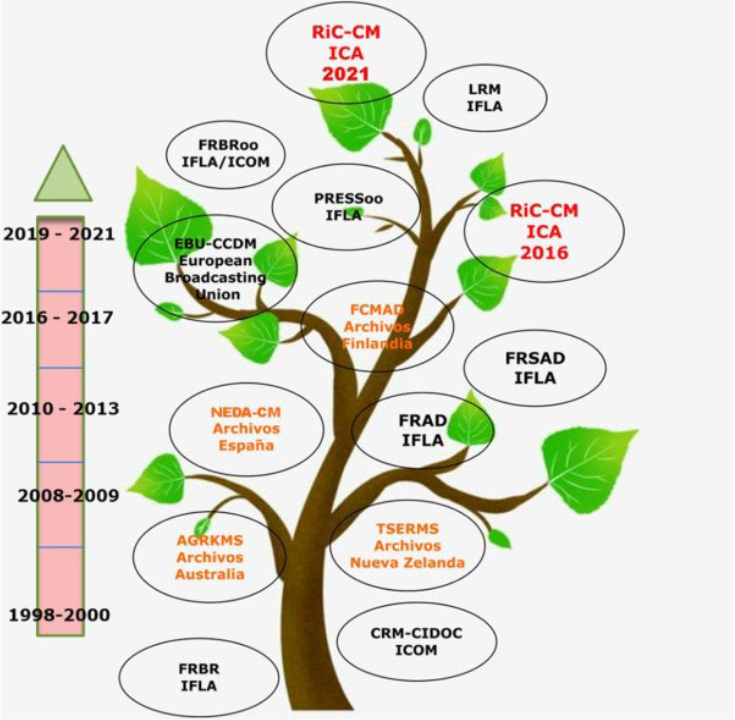
\includegraphics[scale = 0.4]{evolution_CM.png}
    \caption {L'évolution des modèles conceptuels/sémantiques. Issu de D. Llanes Padrón et M. Moro Cabero.}
    \label{fig:enter-label}
\end{figure}
\newline
\subsection{Le \textit{Record in Contexts standard}}
Présenter les deux version du RIC et le RIC-O, les défis et applications déjà en place
\section{L'application de modèles de données ontologiques pour les archives}
\section{Conclusion}

\end{document}
